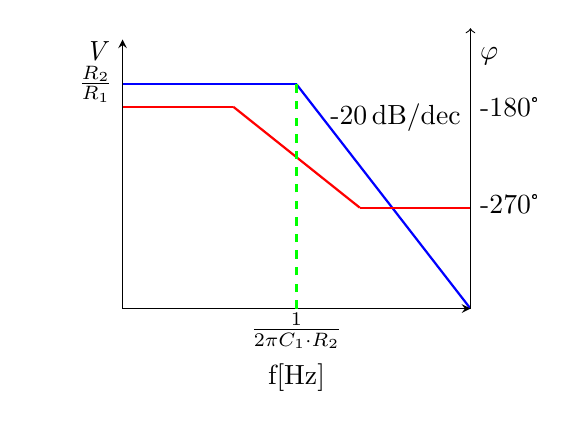
\begin{tikzpicture}[scale=1, transform shape]
    \begin{axis}[
       width=6cm, % Breite des Graphen
       height=5cm, % Höhe des Graphen
        xmin=0, xmax=11,
        ymin=0, ymax=1.2,
        axis lines=center,
        axis on top=true,
        domain=0:10,
        xtick=\empty,
        ytick=\empty,
        ylabel style={xshift=-0.6cm, yshift=0.1cm },
       ylabel={\it V},
       xlabel style={yshift=-0.4cm },
        xlabel={f[Hz]},
        clip mode=individual, % Verhindert das Abschneiden von Elementen
        xlabel style={at={(axis description cs:0.5,-0.05)},anchor=north}
        ]

        \path[draw=none] (axis cs:-3, 0) rectangle (axis cs:13,1);



        \addplot+[mark=none, thick, blue] coordinates {(0,1) (5.5,1)};
        \addplot+[mark=none, thick, blue] coordinates {(5.5,1) (11,0)};
        \node[anchor=east] at (axis cs:0,1) {$\frac{R_2}{R_1}$};
       \node[anchor=east] at (axis cs:11,0.85) {-20\,\text{dB/dec}};
    \end{axis}
    
    \begin{axis}[
       width=6cm, % Breite des Graphen
       height=5cm, % Höhe des Graphen
       xmin=0, xmax=11,
       ymin=0, ymax=240, 
       axis y line*=right,
       axis x line=none,
       ylabel={$\varphi$},
       ylabel style={rotate=270, anchor=west, yshift=1.5cm},
       xtick=\empty,
       ytick=\empty,
       clip mode=individual, % Verhindert das Abschneiden von Elementen
       after end axis/.code={
           \draw[->] (axis cs:11,240) -- (axis cs:11,250);
       }
        ]
        \addplot+[mark=none, thick, red] coordinates {(0,180) (3.5,180)};
        \addplot+[mark=none, thick, red] coordinates {(3.5,180) (7.5,90)};
        \addplot+[mark=none, thick, red] coordinates {(7.5,90) (11,90)};
        \addplot+[mark=none,dashed, thick, green] coordinates {(5.5,0) (5.5,200)};
        \node[] at (axis cs:5.5,-20) {$\frac{1}{2 \pi C_1 \cdot R_2}$};
        \node[anchor=west] at (axis cs:11,180) {-180°};
        \node[anchor=west] at (axis cs:11,93) {-270°};
    \end{axis}
    \end{tikzpicture}